\chapter{Entering expenses in a financial setting}\label{ch:Study1}
\begin{mynote}
\subsubsection{Chapter outline}

In this chapter I describe the findings of an explorative interview study about data entry in a financial work setting. The aim of this study was to get a better understanding of the type of data entry task people at finance offices conduct, and the physical environment in which this is done.
A second planned study is described, that aims to investigate the information sources finance office workers need for an expenses task, and how they currently manage subtasks of looking up information.

\end{mynote}

\section{Study 1: Understanding data entry work in a financial office}\label{ch:Study1}
 
\subsection{Introduction}
As data entry is a common task and it is important this is done both accurately and efficiently, work has been done to design and optimise data entry interfaces to support fast and accurate data entry \citep[e.g.][]{Oladimeji2013, Vertanen2015, Wiseman2013a}.
However, it is not just the input method that determines efficiency and accuracy but also other aspects of the task, such as the environment within which it is conducted \citep{Payne2013, Randall2014}.

\citet{Evans2012} looked if people's text entry and mouse pointing behaviour in a lab setting was comparable to how they would normally perform these inputting tasks in their everyday life. They remotely observed people's input behaviour on their personal computer, and compared this with their performance on similar tasks in a lab. Participants installed a tool on their personal computer which logged all text entry and mouse pointing behaviour they performed in one workweek. Examples of tasks that were carried out were sending personal messages to friends and browsing the web. There were no differences in uncorrected errors or text entry speed between the lab and the field, but they did find that participants corrected more errors in the lab. This study shows that people check and correct their entries more when they are in a controlled environment and are focused on the task, though the measured behaviour on people's personal computers mostly included tasks where accuracy may not have been considered important, such as sending an informal chat message to a friend. 

In order to support people in their data entry work, it is important to first have a better understanding of the types of data entry tasks they have to conduct, and the physical environment in which this is done. Therefore, the first study of this thesis is an explorative study. I visited and interviewed people who conduct data entry tasks as part of their daily work in the finance departments of two universities. This user group was chosen as they have a lot of data entry tasks as part of their job, and it is an area where it is important to enter data accurately, but there is also time pressure to finish work on time. Furthermore, it was an accessible user group to approach for the researcher.

Previous research has given us a good understanding of which factors may influence people's performance on a data entry task. The current study aims to study how these factors are laid out in an applied setting. Furthermore, this study gives an opportunity to see if there are additional problems that influence data entry performance, that are currently not acknowledged in existing literature. 

\subsection{Method}
\subsubsection{Participants}
Nine participants (four male) took part in the study. They were employees from two public universities and their work involved receiving various requests for payment, checking the information of these requests was correct, and entering the information along with administration data into computer systems. Ages ranged from 18 to 52 (two participants wished to not disclose their age). Their level of experience differed, with some participants having just started doing this type of job and other participants working in Finance for 17 years. All but one worked full-time. Table \ref{table:ch3_participants} shows further demographic details of the participants. Typical tasks participants dealt with were checking and entering expense forms sent by staff and students, paying salaries and pensions, controlling research budgets, monitoring university income and expenses and entering employee information. Participants were recruited by sending invitations to opt-in mailing lists of Finance departments, and were reimbursed with a \pounds10 Amazon voucher.

\begin{table}[htp]
\centering
\resizebox{\textwidth}{!}{%
\begin{tabular}{llllllll}
{\bf ID} & {\bf Age} & {\bf Gender} & {\bf Nationality} & {\bf Occupation}                                                             & {\bf University} & {\bf \begin{tabular}[c]{@{}l@{}}Experience in\\ Finance\\ (y = years,\\ m = months)\end{tabular}} & {\bf Deals with}                                                                                     \\ \hline
P1       & 49        & M            & Danish            & \begin{tabular}[c]{@{}l@{}}Research\\ Services\\ Administration\end{tabular} & A                & 17y                                                                                               & \begin{tabular}[c]{@{}l@{}}invoices,\\ statements,\\ grants\end{tabular}                             \\
P2       & 39        & F            & British           & Administrator                                                                & A                & 2y                                                                                                & \begin{tabular}[c]{@{}l@{}}funding,\\ expenses,\\ room\\ bookings,\\ events\end{tabular}             \\
P3       & 20        & F            & British           & \begin{tabular}[c]{@{}l@{}}Credit\\ Controller\end{tabular}                  & A                & 7m                                                                                                & \begin{tabular}[c]{@{}l@{}}money that\\ comes in,\\ payments\end{tabular}                            \\
P4       & -         & M            & British           & \begin{tabular}[c]{@{}l@{}}Assistant\\ Accountant\end{tabular}               & A                & 15y                                                                                               & \begin{tabular}[c]{@{}l@{}}research\\ budgets,\\ expenses\end{tabular}                               \\
P5       & 33        & F            & British           & \begin{tabular}[c]{@{}l@{}}Accounts\\ Assistant\\ Expenses\end{tabular}      & A                & 4y2m                                                                                              & \begin{tabular}[c]{@{}l@{}}expenses,\\ employee\\ information,\\ supplier\\ information\end{tabular} \\
P6       & 18        & M            & British           & \begin{tabular}[c]{@{}l@{}}Payroll and\\ Pensions\\ Apprentice\end{tabular}  & B                & 6m                                                                                                & \begin{tabular}[c]{@{}l@{}}salaries,\\ expenses,\\ pensions\end{tabular}                             \\
P7       & 40        & F            & British           & \begin{tabular}[c]{@{}l@{}}Payroll and\\ Pensions\\ Assistant\end{tabular}   & B                & 10y                                                                                               & \begin{tabular}[c]{@{}l@{}}salaries,\\ expenses,\\ pensions\end{tabular}                             \\
P8       & 52        & M            & British           & \begin{tabular}[c]{@{}l@{}}Payroll\\ Supervisor\end{tabular}                 & B                & 12y                                                                                               & \begin{tabular}[c]{@{}l@{}}salaries,\\ expenses,\\ pensions\end{tabular}                             \\
P9       & -         & F            & British           & Payroll Officer                                                              & B                & 13y                                                                                               & \begin{tabular}[c]{@{}l@{}}salaries,\\ expenses,\\ pensions,\\ employee \\ information\end{tabular} 
\end{tabular}
}
\caption[Study 1 participant information]{Participant information.}
\label{table:ch3_participants}
\end{table}

\subsubsection{Materials}
Materials that were used during the interview were a voice recorder, a paper copy of an interview script with the interview topics and guiding questions, a consent form, an information sheet for the participant and a notebook and pen to make notes. The interview script, information sheet and consent form are included in the Appendix. 
Each interview covered four guiding topics, which are briefly described in Table \ref{table:ch3_interviewtopics}. For each topic, a number of questions were written out beforehand. These questions were used as a starting point to get the participant talking and guide the interview. Based on what the participant was saying follow-up questions were asked. The audio transcription program ExpressScribe was used to transcribe the interviews. The data analysis programs Nvivo and Atlas.ti were used to analyse the data. Nvivo was used to code the interview transcripts and notes. Atlas.ti was used to complement the analysis in Nvivo and allowed to identify relations between codes.

\begin{table}[htp]
\centering
    \begin{tabular}{ | l | p{10cm} |}
    \hline
     Topic & Description \\ \hline
    Job description & A description of the tasks that the interviewee deals with. The purpose of this topic was to start the interview easy and give the interviewee the opportunity to explain what their job entails. \\ \hline
    Number transcription & This includes questions on when and how people typically enter numbers for work.  \\ \hline
Environment & This topic includes people's physical work environment, and the organisation they are a part of. \\ \hline
Demonstration &  Interviewees were asked to give a demonstration of entering data into their system. The aim of this part of the interview is to see the type of data entry tasks people have to do, and also gives a chance to see the information sources and systems people currently use. \\
    \hline
    \end{tabular}
    \caption[Study 1 interview topics]{Interview topics.}
    \label{table:ch3_interviewtopics}
\end{table}%

\subsubsection{Data recording}
A voice recorder was used to audio record the interviews. One participant wished to not be audio recorded and one interview could not be audio recorded due to technical issues, so for these two interviews notes were taken of the answers. For the remaining seven interviews, notes were only made of observations and not the participants' answers. Notes were made with pen and paper. Photographs were made of the work environment and screenshots of the systems that the interviewees used.

\subsubsection{Interviewing procedure}
The interviews took place at the participants' workplace. For two interviews, the interviewee's office place was not suitable for talking so the interview took place in a common room nearby, and these participants showed their workplace and completed a demonstration of entering data after the interview. 
Participants were welcomed and informed about the study. They received a paper information sheet with the outline of the study and contact details of the researcher to keep for future reference. They were also asked to read and sign a consent form.

The interviews were semi-structured and took between 20 and 55 minutes. Each interview was reviewed afterwards, and findings sometimes fed into new questions being included or some questions being adapted in subsequent interviews.

\subsubsection{Pilot interview}
A pilot interview was conducted with an acquaintance of the researcher who worked in Finance, to test out the set-up of the study and questions. The interview took place at the participant's home, notes were taken with pen and paper, and the interview was audio-recorded using iMovie on a Macbook Pro. 

Taking notes slowed down the flow of the interview: sometimes the interviewee stopped talking to give the interviewer the opportunity to finish taking notes. Furthermore, taking notes took attention away from what the interviewee was explaining: assumptions made during the interview did not seem to be accurate in later analysis. Therefore, it was decided that note taking would be kept to a minimum. Notes would only be made of observations that could not be taken from audio recordings.

The interviewee talked elaborately about manually converting different currencies, and identified this task as the main place where errors occurred. Therefore, questions were included about if interviewees dealt with foreign currencies and converting these. 

\subsubsection{Ethical considerations}
The study was undertaken with ethical approval from the UCL Research Ethics Committee [Project ID Number UCLIC/1415/001/Staff Brumby/Borghouts]. 
At the start of each interview, participants were first informed verbally about the study. They were then given a consent form to read and sign, and were given an information sheet to keep. This information sheet contained the study information and contact details of the researcher and the project's principal researcher, should participants have any further questions after completion of the study.  They were asked permission for the interview to be audio recorded. One participant wished not to be audio recorded and notes were taken instead. 

Participants were informed that the data would be used for research purposes only and stored in accordance with the Data Protection Act 1998. They were also informed that their data would be anonymised and when used in a report or academic paper, their data would not be directly identifiable. Names of participants or the universities they were working at were not included in the interview notes and transcripts.
 
\subsection{Results}
\subsubsection{Data analysis}
After each interview or set of interviews, a first analysis took place. The audio recording was played back, notes were typed into a digital file and reviewed and the interview was transcribed verbatim. Several non-verbal cues were included in the transcription as well, such as when the interviewee laughed or sighed, as well as descriptions of when the interviewee was demonstrating something. The advantage of doing the transcription shortly after the interview was that it was still easy to remember from listening to the audio recording what was being demonstrated. Interesting findings and initial patterns that were apparent across the data were written down. 

After all interviews had been transcribed, the transcriptions and notes were printed and the data was analysed using thematic analysis \citep{Braun2006}. Anything in the data that was considered to be interesting was annotated by hand and labelled with an appropriate code. On reviewing the coding, some codes were grouped together in one code, additional codes were named, and similar codes were grouped under themes. For instance, an initial code was Notifications, such as e-mail notifications. During the second coding iteration, it was identified that people always talked about notifications in the context that they were interrupted (by a notification) rather than about notifications on its own. Therefore, notifications and interruptions were grouped into one code. 

The themes were then reviewed, to see if they addressed the purpose of the study. The transcripts and notes were then imported into Nvivo and coded digitally. Atlas.ti was used to complement this analysis and allowed to identify relations between codes. 

\subsubsection{Themes}
In total 51 codes were derived, and these were grouped into 8 main themes, which are listed and described in Table \ref{table:ch3_themes}. If codes or separate quotes did not belong in a certain theme but were still considered relevant, they were grouped in the Other category. 

\begin{table}[htp]
\centering
\resizebox{\textwidth}{!}{
    \begin{tabular}{ | p{3cm} | p{8cm} | l | l |}
    \hline
     \textbf{Theme} & \textbf{Description} & \textbf{Quotations} & \textbf{Participants} \\ \hline
     Task characteristics & People described things that were particular to their task, for instance how they structured their task, whether they switched tasks, and how long they took to complete tasks.  & 129 & 9 \\ \hline
	 Checking & People talked about checking data input as part of their job. & 103 & 9 \\ \hline 
	System & People talked about the computer system they were using to input data.  & 91 & 9 \\ \hline 
		Environment &People described their environment, for instance they talked about their physical work setting, and the work culture of their organisation. & 80 & 9 \\ \hline 
		Data &People described the data they were dealing with, for instance the type and length of data items, and from which source they copied data. & 75 & 9 \\ \hline 
		Errors &People described situations where errors were made: who made them, why were they made, what were the consequences. & 75 & 9 \\ \hline 
					 Strategy & People described the strategies they used to carry out their task.  & 54 & 9 \\ \hline 
		Importance of accuracy and paper trails &People talked about the sensitivity of financial data which is why not all people are authorised to approve or access financial data, and the importance of a paper trail for data entries. & 35 & 8 \\ \hline 
			 			 Other & People talked about things that did not fit into any other category but were still considered relevant, such as issues they experienced, or queries they often received.   & 74 & 9 \\ 
    \hline
    \end{tabular}
    }
    \caption[Study 1 Themes]{The themes, along with a description. The column Quotations indicates how many times this theme was brought up during interviews, and the column Participants indicates how many participants talked about it.}
    \label{table:ch3_themes}
\end{table}

Each theme is described separately in subsections below, and is visualised in a diagram, which shows the theme's main codes and relationships between codes, as well as quotes in dotted squares to exemplify what type of quotes were grouped under this code. The numbers in parentheses indicate the number of quotes, and the number of interviewees who mentioned it. 
The description of each theme is accompanied with notes and quotes taken from the transcripts to further illustrate when this theme was mentioned. These serve as examples and are not all the instances of a theme. To differentiate notes from verbatim quotes, the quotes are in italics and double quotation marks. Words put in brackets are added by the researcher to make the quote more understandable for the reader, for instance if the interviewee is talking about 'it' or 'them'.
The results are ordered according to the number of quotations associated with a theme, with the theme with the most quotations listed first. The only exception is the 'Other' theme which is described last.
\newpage
\subsubsection{Task}
\begin{figure}[!ht]
\centering
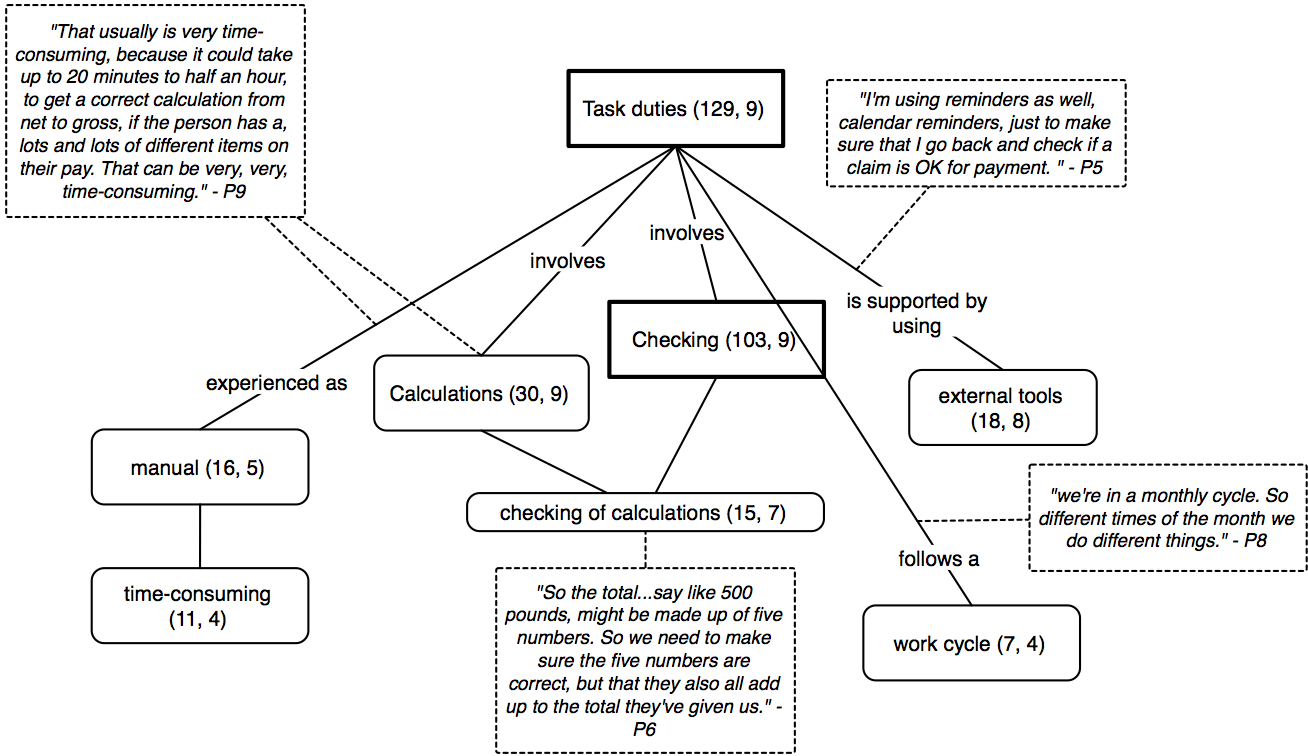
\includegraphics[width=\textwidth]{images/Study1/Task.png}
\caption[Study 1 Task diagram]{Diagram showing the theme Task. The numbers in parentheses indicate the number of quotes and the number of participants who mentioned it, respectively.}
\vspace{-9pt}
\label{fig:ch3_task}
\end{figure}
A common data entry task was entering expenses. Interviewees received expense claims from students and staff and had to check the information was correct. They then had to enter this data, along with other information such as budgetting and staff information, into a computer system.
All interviewees mentioned a large part of their job was checking that data was correct. In addition to transcribing and checking individual numbers, participants also mentioned they often have to perform and check calculations.
 Some tasks, such as calculations, had to be done manually and this was described as time-consuming. People used several external tools in their environment to support them in their tasks. For instance, P7 and P8 had paper sheets on their desk with information they frequently had to look up, so they could easily use this to check if the input they had received was correct.

Some people worked according to a work cycle, which meant they did different things at different times of the month. One week could be reserved for checking all the data they received from another department, while another week could be spent on solely inputting data. 

The time spent on each task differed: checking data on a short expenses form could be completed in two minutes, while a single calculation could take between 20 and 30 minutes. Two participants experienced dealing with a lot of data entry as tiresome.

\newpage

\subsubsection{Checking}\label{subsec:Checking}
\begin{figure}[!ht]
\centering
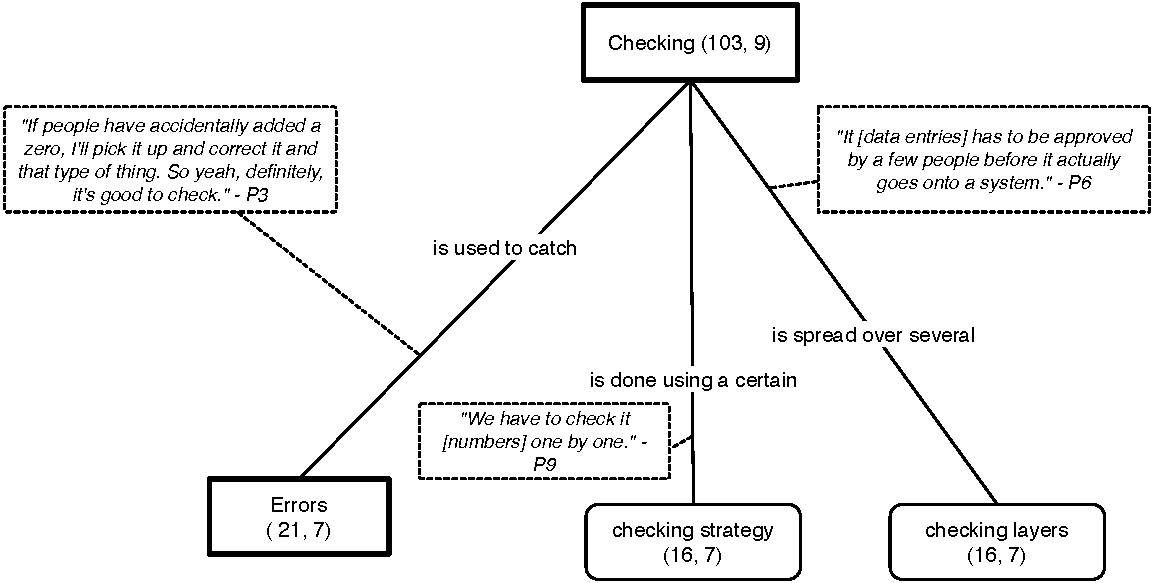
\includegraphics[width=\textwidth]{images/Study1/Checking.pdf}
\caption[Study 1 Checking diagram]{Diagram showing the theme Checking.}
\vspace{-9pt}
\label{fig:ch3_checking}
\end{figure}

All participants talked about checking data input for errors as a part of their job. Data was checked by several different people and departments before it was submitted. People's experience with this checking system differed: P3 felt that an error would be caught eventually because it goes through so many different layers, whereas P9 said it made people less careful about making errors and therefore they often received erroneous data. Sending wrong input back slowed the process down, and P8, who acted as the last person in his department to check before it gets submitted, warned that even with extra human checks not all errors get caught. 

People had to both check their own data input, as well as double-check other people's input. They maintained different checking strategies, ranging from checking each data item one by one to entering a group of data items first and then checking. 


\begin{table}[htp]
\centering
    \begin{tabular}{ | l | p{10cm} |}
    \hline
     \textbf{Participant} & \textbf{Quote} \\ \hline
    P3 & \textit{"we try and pick it [errors] up and then obviously there's all the different stages that pick it up as you go along."}\\ \hline
    P9 & \textit{"the departments actually sometimes treat us as a checking system [laughs], but they shouldn't really, the schools. Because we're here just to make sure that people get paid correctly. But even though we are like a second check, we feel sometimes that we are the first checkpoint."} \\ \hline
    P7 & \textit{"All this piece of work, when we input in the system, will be actually checked by another person... my manager will print it out, and then check... other colleagues will double-check it for you as well, the calculations."} \\ \hline
    P8 & \textit{"one of these errors could be things that are missed during the checking."} \\ \hline

    \hline
    \end{tabular}
    \caption[Study 1 checking quotes]{Verbatim quotes taken from the interview transcripts that were about checking.}
    \label{table:ch3_checkingquotes}
\end{table}%

\begin{table}[htp]
\centering
    \begin{tabular}{ | l | p{10cm} |}
    \hline
     \textbf{Participant} & \textbf{Quote/note} \\ \hline
    P1 &  first puts in all the details, then when done checks everything against the source. \\ \hline
    P7 & when entering numbers from paper to computer, mostly looked at paper form and the number pad; only looked at screen after finishing entering all the numbers from the form to check. \\ \hline
    P5 & \textit{"We would go by the receipt, so we would try to make sure that the receipts are in order."} \\ \hline

    \hline
    \end{tabular}
    \caption[Study 1 checking own input]{Checking own input when entering data.}
    \label{table:ch3_owninputquotes}
\end{table}%

\begin{table}[htp]
\centering
    \begin{tabular}{ | l | p{10cm} |}
    \hline
     \textbf{Participant} & \textbf{Quote} \\ \hline
    P5 &  \textit{"The numbers on the expense form will be checked individually. So the total will obviously be, say like 500 pounds, might be made up of five numbers. So we need to make sure the five numbers are correct, but that they also all add up to the total they've given us."} \\ \hline
    P6 & \textit{"The numbers on the expense form will be checked individually."}\\ \hline
    P9 & \textit{"We have to check it one by one."} \\ \hline

    \hline
    \end{tabular}
    \caption[Study 1 checking other people's input]{Checking other people's input.}
    \label{table:ch3_otherinputquotes}
\end{table}%

\clearpage
\subsubsection{System}
\begin{figure}[!ht]
\centering
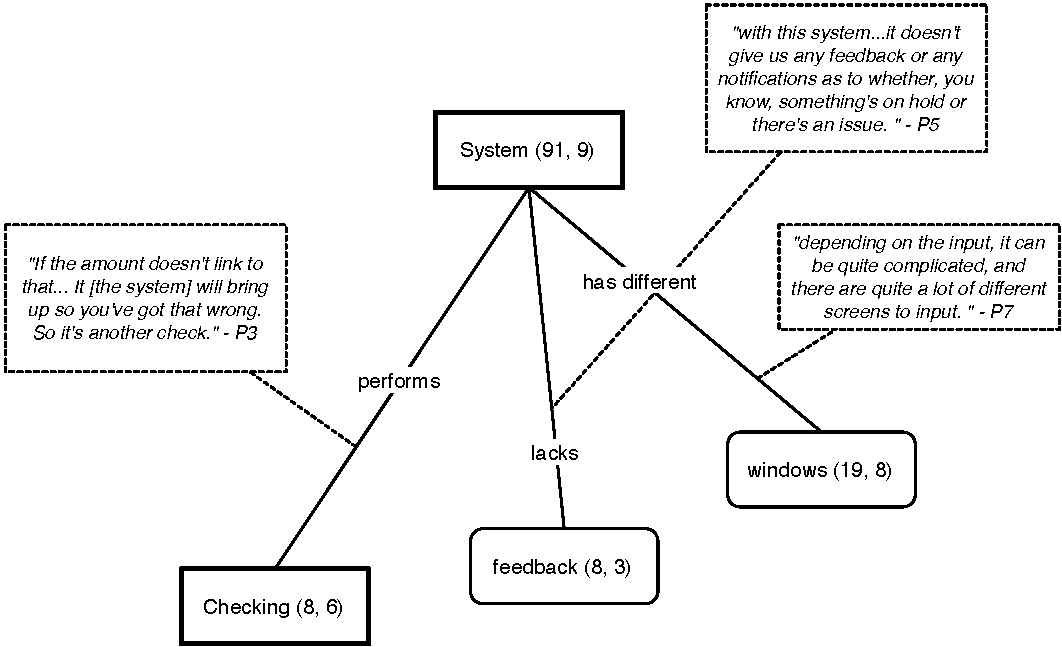
\includegraphics[width=\textwidth]{images/Study1/System.pdf}
\caption[Study 1 System diagram]{Diagram showing the theme System.}
\vspace{-9pt}
\label{fig:ch3_system}
\end{figure}

Data had to be entered into an information system on a computer. Some participants mentioned the system was another way to check for erroneous data entries: if the allowed number range of a variable was known, the system would let the user know if an out-of-range number was entered. However, it was also mentioned that one issue with the financial data entry system was that it did not give feedback if there was an issue or error.

The information needed for one task was usually spread over several windows on the computer, so sometimes people had to flick back and forth or memorise certain information from one window to use in another window. 

\clearpage
\subsubsection{Environment}
\begin{figure}[!ht]
\centering
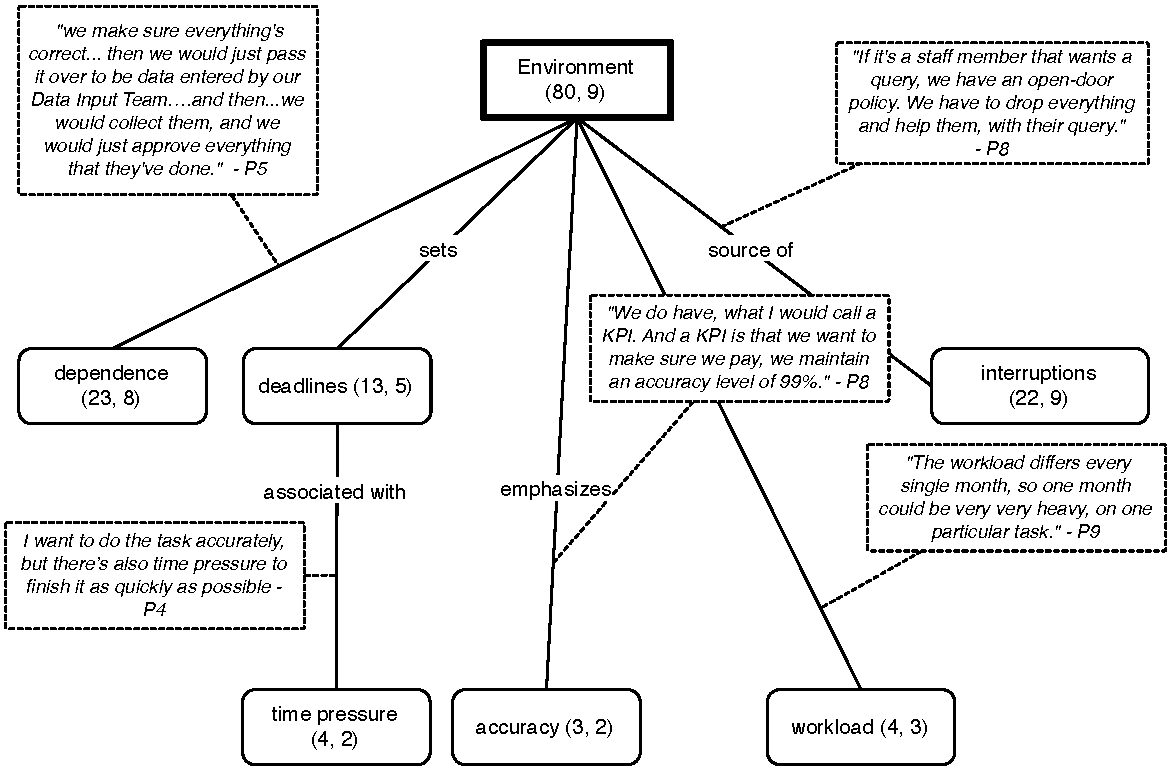
\includegraphics[width=\textwidth]{images/Study1/Environment.pdf}
\caption[Study 1 Environment diagram]{Diagram showing the theme Environment.}
\vspace{-9pt}
\label{fig:ch3_environment}
\end{figure}

Every time people described the environment they were working in, this was grouped under the Environment theme. The environment could be their immediate physical setting, or their organisation in general. 

All participants experienced interruptions during work. P8 mentioned he had to pause his task immediately if a staff member needed his help, but considered these interruptions part of his job. Other interviewees mentioned they tried to concentrate on the task at hand first, but did briefly attend to interruptions such as e-mail notifications, in case it was important.

People were dependent on other departments to finish a task. For instance, P5 checked paper expense forms, but did not enter these into the system herself. 

Some participants felt the pressure to be both accurate in data entry, as well as finish it quickly because of deadlines. The workload varied throughout the year.

\newpage
\subsubsection{Data}
\begin{figure}[!ht]
\centering
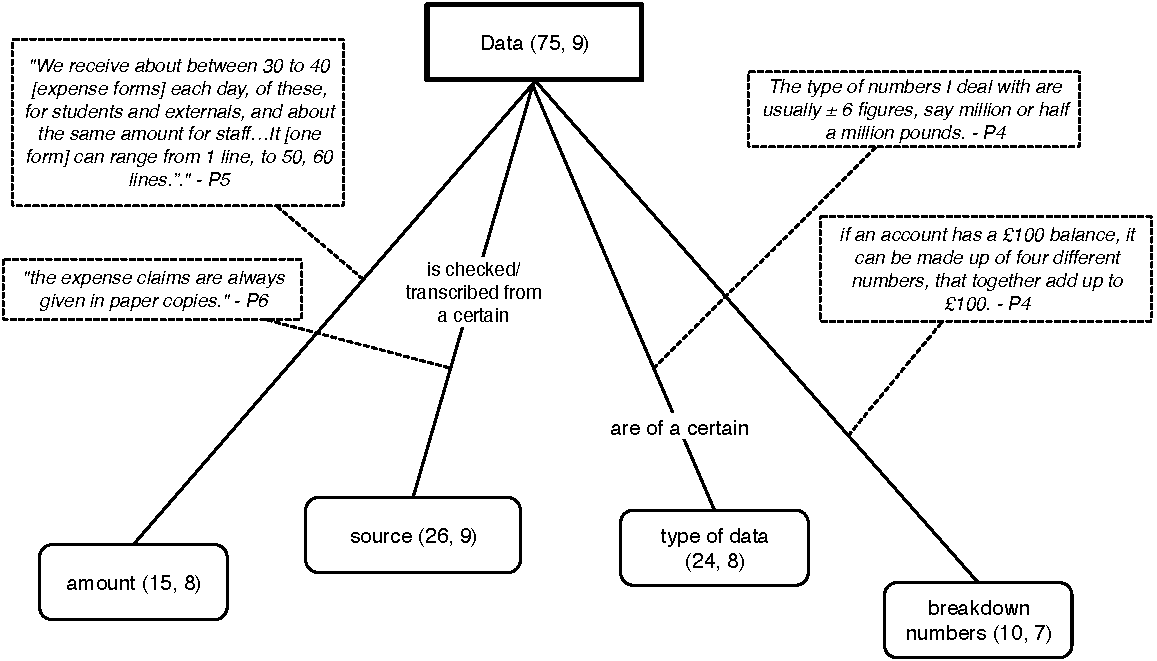
\includegraphics[width=\textwidth]{images/Study1/Data.pdf}
\caption[Study 1 Data diagram]{Diagram showing the theme Data.}
\vspace{-9pt}
\label{fig:ch3_data}
\end{figure}

Participants had to retrieve data from various sources. Some of the sources were electronic, such as Excel spreadsheets and Word documents. Some information had to be looked up in databases and work e-mails. Other information was received on paper sheets, and some participants had printed out information they frequently needed and had placed this on their desk. People had to transcribe numbers from paper onto a computer system for at least a part of their tasks. Some people worked with two screens.
The amount of data that people dealt with differed. P5 said that for expenses alone, the amount of numbers she received each day to check and input ranges from 100 to 6000 numbers.
People primarily dealt with numeric data, such as financial data and IDs. The monetary numbers they dealt with ranged from five to millions of pounds. Participants also entered and checked alphanumeric and non-numeric data such as employee names, addresses and bank account details.

Numeric data consisted of individual numbers, as well as groups of numbers that together made up a new number, such as the total amount of money spent on a project. Participants had to both check and transcribe each individual number, and check that the calculation was correct. 

\ \clearpage

\subsubsection{Errors}
\begin{figure}[!ht]
\centering
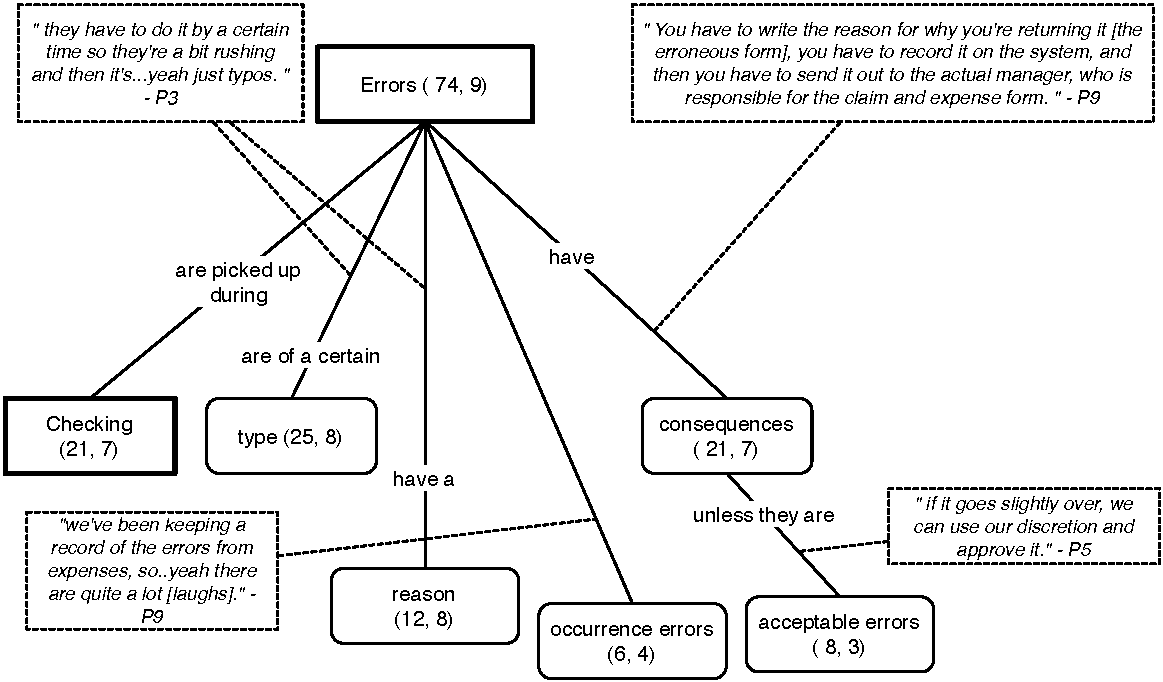
\includegraphics[width=\textwidth]{images/Study1/Errors.pdf}
\caption[Study 1 Errors diagram]{Diagram showing the theme Errors.}
\vspace{-9pt}
\label{fig:ch3_errors}
\end{figure}

Participants discussed that errors happened frequently, and talked about errors they spotted from other people. Visual checking was mentioned as the main method to catch and correct errors in time, but when possible the computer system sometimes checked for erroneous data as well. Errors that were made were typos, miscalculations, or people had the wrong information to enter. For instance, P7 mentioned that when salary rates change, employees often keep entering their old salary rate on claim forms, which then has to be corrected. The main explanation people gave for errors was that it is human to make mistakes, but it was also mentioned people are under time pressure, and that people rely on the fact it will be checked by another person, which makes them less careful in entering accurate data. 
If an error was spotted, this had certain consequences depending on if the error was acceptable or not. If the error was sufficiently small, it could be either processed or corrected without negotiation, but if it was a large error, it had to be sent back or forwarded to a higher authority for approval. 

P1 highlighted project IDs used to be letters but are now numbers, which are harder to memorise, and he felt it was easier to make a mistake. P4 worked with both paper and digital files to transcribe data from, but preferred digital files because he felt it was much easier to make an error and omit figures when transcribing from paper.

\begin{table}[htp]
\centering
    \begin{tabular}{ | l | p{10cm} |}
    \hline
     \textbf{Participant} & \textbf{Quote/note} \\ \hline
    P6 &  \textit{"it's quite common that we have to return an expense or payment back to someone. It happens quite often, yeah."} \\ \hline
    P4 & Yes all the time, lots of typos.\\ 
    \hline
    \end{tabular}
    \caption[Study 1 errors quotes]{People mentioned errors occur quite frequently.}
    \label{table:ch3_occurrenceerrorsquotes}
\end{table}%


\begin{table}[htp]
\centering
    \begin{tabular}{ | l | p{10cm} |}
    \hline
     \textbf{Participant} & \textbf{Quote} \\ \hline
    P3 &  \textit{"sometimes it's because people have done typos, done too many zeroes, or left out a zero."} \\ \hline
    P5 & \textit{"the expense breakdown doesn't match what (...) whatever they put as the grand total."}\\ 
    \hline
    \end{tabular}
    \caption[Study 1 type of errors quotes]{The type of errors.}
    \label{table:ch3_typeoferrorsquotes}
\end{table}%


\begin{table}[htp]
\centering
    \begin{tabular}{ | l | p{10cm} |}
    \hline
     \textbf{Participant} & \textbf{Quote} \\ \hline
    P9 &  \textit{"Because the departments actually sometimes treat us as a checking system [laughs], but they shouldn't really."} \\ \hline
    P7 & \textit{"Yeah, human laziness or something [laughs]."}\\ \hline
    P8 & \textit{"sometimes, you know, through human error, you know, things don't get paid properly."} \\
    \hline
    \end{tabular}
    \caption[Study 1 reasons for errors quotes]{The reasons for errors.}
    \label{table:ch3_errorreasonsquotes}
\end{table}%


\begin{table}[htp]
\centering
    \begin{tabular}{ | l | p{10cm} |}
    \hline
     \textbf{Participant} & \textbf{Quote/note} \\ \hline
    P5 &  \textit{"generally we tend, we try not to send claims back to departments because they might get lost in the post, and it's an inconvenience as well. So we try to... resolve it ourselves.."} \\ \hline
    P4 & We allow a certain amount of tolerance; if it turns out the thing you bought has actually decreased value and is now  \pounds40, we will allow to return  \pounds50\\ \hline
    P7 & \textit{"we normally e-mail the budget holder to say... what you authorised is actually different. But for this kind of thing, it's only 10 pounds...we normally just process this without contacting them."} \\ \hline

    \hline
    \end{tabular}
    \caption[Study 1 acceptable errors quotes]{Acceptable errors.}
    \label{table:ch3_acceptableerrorsquotes}
\end{table}%

\clearpage
\subsubsection{Strategy}
\begin{figure}[!ht]
\centering
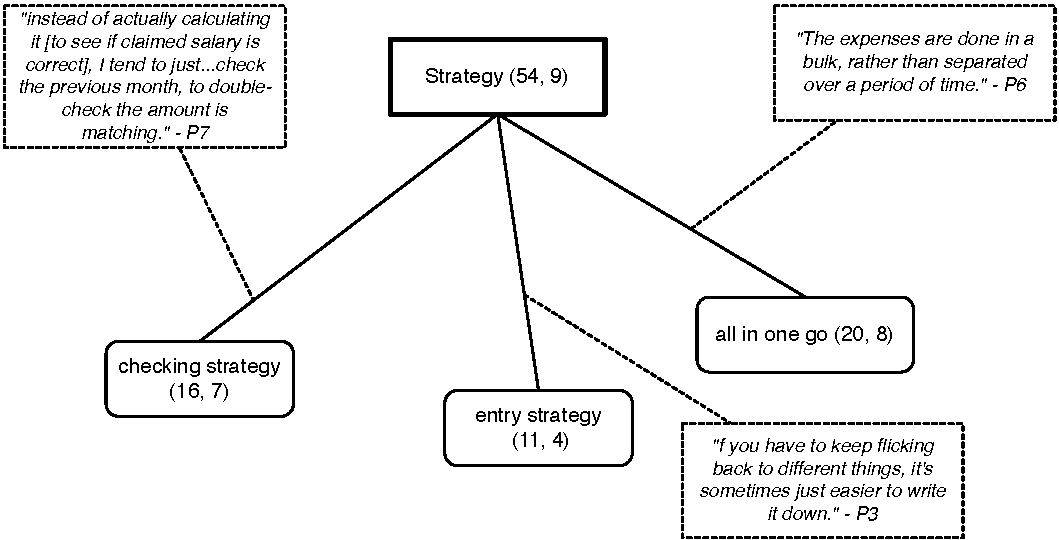
\includegraphics[width=\textwidth]{images/Study1/Strategy.pdf}
\caption[Study 1 Strategy diagram]{Diagram showing the theme Strategy.}
\vspace{-9pt}
\label{fig:ch3_strategy}
\end{figure}

Eight of nine interviewees saved up data to enter it all in one sequence. If they received forms with data input to check or enter, they saved these for later and then processed all the forms. P1 indicated he processed forms in batches of at least five forms, and found it disruptive to do just one or two and then switch to something else. 

P2 was the only interviewee that processed forms with numbers to enter as they came in, but did admit that if she had more data to fill in, she would probably do it in a more efficient way.

Some people said they preferred batching their work so that they entered all data into a single system at once because it is quicker and easier to do the same type of tasks in one sequence, and when that is finished concentrate on another task. P4 mentioned he does them all at once because he gets the forms in a bulk and feels pressure by his boss to finish them all immediately, rather than spread them over time. P6 explained he postpones processing expense forms until the deadline to submit forms for that month has passed, after which he does all forms in one sequence. 

People also talked about other strategies they used to do their job more efficiently. For instance, if they had to get out of the system to look up information digitally and then get back to the system window to enter it, they preferred to memorise the information, rather than flick back and forth and look it up each time they needed it. With numbers they had to enter frequently such as project codes, they memorised it even if they did not deliberately choose to do so. If the information to remember was complicated, they would write it down.

As discussed at the \nameref{subsec:Checking} section, people had different checking strategies and the number of times they looked back to the data source to check it against the data input varied. P7 said she sometimes deals with similar calculations, so she prefers to check the calculation she did last time rather than calculate it again. 

People explained that a lot of numbers they enter are calculated from other numbers. Some people liked to write out and keep a record of their calculation, in case someone had any questions on how that number was calculated.

\begin{table}[htp]
\centering
    \begin{tabular}{ | l | p{10cm} |}
    \hline
     \textbf{Participant} & \textbf{Quote/note} \\ \hline
    P3 &  \textit{"I just try and do it in the quickest way...It's nice, once you've done it, it's completed, so it's sort your weight lifted [laughs]. So you don't need to think about it again."} \\ \hline
    P6 & \textit{"the expenses are done in a bulk, rather than separated over a period of time. When I'm doing it lots at a time, I think once you get into sort of the hang of it, it gets done a lot quicker than..you just get used to putting them in, and inputting it all."} \\ \hline
    P9 & \textit{"I try to concentrate on my task...I try to do one task [i.e. doing all expenses], finish one, and then do another."} \\ \hline
    P4 &  It's difficult to take rests or even switch in-between number entry tasks because of the work pressure, and feels pressure by boss. \\ 
    \hline
    \end{tabular}
    \caption[Study 1 batching quotes]{Most participants entered all numbers in one go.}
    \label{table:ch3_inonegoquotes}
\end{table}%

\begin{table}[htp]
\centering
    \begin{tabular}{ | l | p{10cm} |}
    \hline
     \textbf{Participant} & \textbf{Quote/note} \\ \hline
    P3 &  \textit{" I wouldn't necessarily have to [memorise numbers], It's more just if you have to keep flicking back to different things, it's sometimes just easier to write it down, or just try and remember it. But you can obviously take the long version and keep flicking back to the correct screen."} \\ \hline
    P2 & \textit{"we have different grants and different project codes as a result, but you, because you use them so much, you end up remembering them."} \\ \hline
    \end{tabular}
    \caption[Study 1 strategy quotes]{Examples of strategies people used.}
    \label{table:ch3_strategiesquotes}
\end{table}%

\ \clearpage

\subsubsection{Importance of accuracy and paper trails}
\begin{figure}[!ht]
\centering
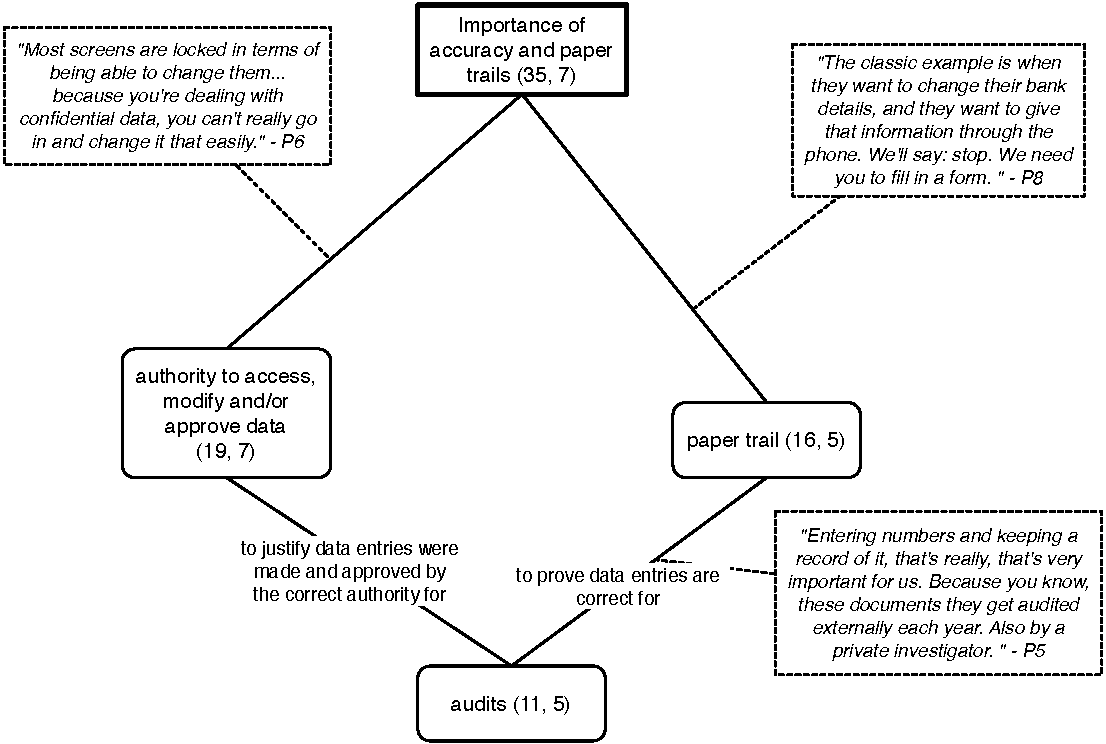
\includegraphics[width=\textwidth]{images/Study1/Papertrail.pdf}
\caption[Study 1 Importance of accuracy and paper trails diagram]{Diagram showing the theme 'Importance of accuracy and paper trails'.}
\vspace{-9pt}
\label{fig:ch3_papertrail}
\end{figure}

Because interviewees were working with sensitive financial data, another theme was importance of accuracy and paper trails.
Some data could only be entered in the system and modified by certain people.
Large figures had to be approved by a superior first before it could be processed, so it was clear to an auditor that expenses were made with the correct approval.
Hard copies of data had to be archived and were checked by external auditors. For instance, all expenses were claimed on paper forms, and had to have the original receipts as evidence that the expense claims were correct. Some data could not be given over the phone but had to be written down and sent via a paper form.

\pagebreak

\subsubsection{Other}
\begin{figure}[!ht]
\centering
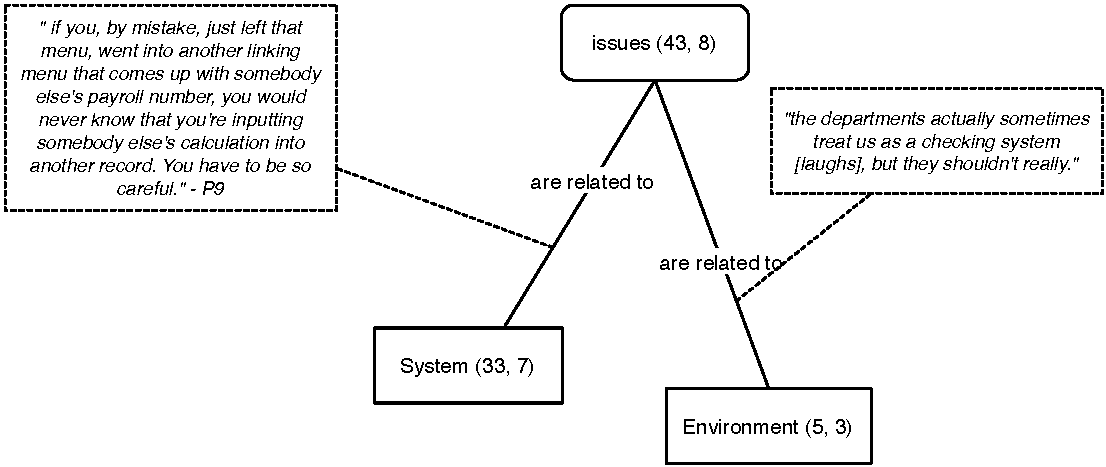
\includegraphics[width=\textwidth]{images/Study1/Other.pdf}
\caption[Study 1 Other diagram]{If people described issues, it usually had to do with the system.}
\vspace{-9pt}
\label{fig:ch3_other}
\end{figure}

Interviewees mentioned several issues they experienced. Most of the time, the issues had to do with the current data entry system they were using. P7 mentioned number entries on the computer screen were small and hard to read, and could not be enlarged. P5 mentioned she did not get notifications from the system if there was an issue with a payment, so she would not know about it until staff members would call up to complain they had not been paid yet.  Other issues had to do with the organisation, such as the experience that the multiple checking layers made people rely on other people to check their input.

\begin{table}[htp]
\centering
    \begin{tabular}{ | l | p{10cm} |}
    \hline
     \textbf{Participant} & \textbf{Quote/note} \\ \hline
    P5 &  \textit{"There are other issues. You could say I think hundreds, I mean not just with the work that we do on expenses, but across [university A], across [university A] Finance, the Finance division...We just have to kind of work our way around the system and you know, adapt to it."} \\ \hline
    P7 & \textit{"It's only the matter of how you get used to the Payroll system. Because companies have different systems, the data inputting can take a while to get used to it."} \\ \hline
    P9 &  \textit{"You know, all systems are a bit funny, I think. But you just gotta get used to it."} \\ \hline
    \end{tabular}
    \caption[Study 1 issues quotes]{Issues that participants experienced with the system.}
    \label{table:ch3_otherquotes}
\end{table}%

\pagebreak

\subsection{Discussion}
The purpose of this study was to gain a better understanding of the type of data entry tasks in financial offices, and the physical environment in which these are conducted. For this purpose nine interviews were conducted with staff from two public universities who worked with financial data. The main findings of the study are: 

\begin{itemize}
\item 
people have to get the data to enter from various sources, with varying information access costs
\item 
people batch their work to enter a lot of data entry at once, and minimise switching between tasks. 
\item 
data entry errors are common, and the current solution is to have data entered and checked by multiple people before it gets submitted to the system
\end{itemize}

\subsubsection{Information sources and access costs}
A prevalent data entry task of participants' work was processing expense claims from university staff and students. A substantial part of this task is not just entering the data but also collecting it from multiple sources. For example, the expenses had to be entered from paper forms and receipts, foreign currencies had to be converted and copied from a website, and staff and financial information had to be retrieved from sources such as electronic spreadsheets, databases and e-mails. 
In data entry experiments, the data is often shown on a computer, to make it easy to manipulate. This was sometimes the case in the office setting studied here, but data was also transcribed from paper sheets into a computer. Furthermore, in lab experiments people are often only presented with the data they have to enter and sometimes are given only one data item at a time. The sources from which people had to enter data in this study usually contained a lot of data, not all of which was relevant to the task. The amount of irrelevant data on the sources can increase the time people need to look up the information they need.

The cost to access the information sources differed. For instance, some paper sheets were on people's desk, but some paper sheets had to be retrieved elsewhere. Sometimes participants had to go through a large spreadsheet, before they found the number they needed to copy. Participants also dealt with multiple windows on their computer screen, and sometimes needed to switch between different windows. Instead of flicking back and forth to view information they had to enter in another window, people said they preferred to memorise it. This supports previous research which showed that people make strategic use of internal and external resources and do not always maximise off-loading cognition to external resources \citep{Gray2006}. Even though participants were aware they did not have to remember information, they found this easier and faster rather than looking it up or writing it down. 

This strategy allows people to be faster, but carries the risk that they misremember it. In previous studies, trying to hold more items in memory during a copying task increased errors \citep[e.g.][]{Morgan2009}. However, in these studies people had to copy over coloured blocks, which were abstract to the participants and may have been too hard for participants to memorise \citep{Waldron2011}. In the current study, the information had some meaning to the users, and even if they were dealing with abstract information, such as project codes or ID numbers, some items were entered more often than others. Participants mentioned that even if they did not make a conscious effort to memorise these, they had to enter these numbers so often that they ended up remembering them. This is in line with prior findings that some numbers are more familiar than others, and that these familiar numbers are more strongly represented in memory \citep{Wiseman2014}. 

If information to copy is familiar and contains numbers and text, making the effort to encode the information more deeply has been shown to make people more accurate \citep{Gray2004, Soboczenski2013}. It is therefore not clear if the effect of a memory-based strategy on accuracy, as found in \citep{Morgan2009}, would extend to copying the material of this study.

People used some external tools to aid memory. For example, some participants had printed sheets with information they used and entered often, so they did not have to repeatedly look this up in the system. They also used calculators and pen and paper to perform calculations.

\subsubsection{Batching data entry tasks}
Eight of nine participants batched data entry tasks to do them all at once, rather than spread them over time. The only participant who processed expense forms as they came in said she did not receive a large amount of forms. She explained that if she dealt with a higher volume of expenses, she would probably do it in a more efficient way.

There were different reasons behind the strategy to enter a large amount of data in one sequence. One participant received forms in a bulk, and felt time pressure to finish them all at once, rather than spread them over time. The other seven participants said they received forms on an ad-hoc basis, but deliberately saved them until a specific moment and then processed them all in a bulk. They preferred to focus on one task at once, and some people stated that it made them faster in entering data after a while. 

This is consistent with Healy et al.'s \citeyearpar{Healy2004} study, where learning effects could be measured in a number entry task. However, in their experiment participants became faster but also more erroneous in entering data. In the current study, P3 mentioned that most of the errors she picks up from colleagues are typos caused by rushing to finish the task. P4 mentioned that he wants to enter numbers accurately, but that there is a time pressure to finish things in time. This is in line with the speed-accuracy trade-off discussed in literature, and that a sense of urgency may cause people to enter numbers faster but at the expense of a higher error rate \citep{Lin2011, Lin2013}.
\citet{Healy2004} recommended regular breaks when entering large amounts of data to maintain accuracy, but P4 in the current study explained it is difficult to initiate breaks himself, when he feels a time pressure to finish it.

\subsubsection{Multiple checking stages}
In order to prevent errors, input was entered and checked by multiple people before it was allowed to be submitted into the system. This checking method is similar to \citeauthor{Reason1990}'s \citeyearpar{Reason1990}  Swiss Cheese model, where multiple checking layers are used to minimise the risk of errors. However, as a result of this people seemed less careful in checking their own input, because they knew it would be checked by someone else. 

In previous studies, providing incentives for people and introducing lockouts into the data entry interface has been shown to influence how carefully people check their input \citep{Li2015, Gould2015}. The findings from the current study suggest that how and whether people check also partly depends on what the primary objective of their task is: entering or checking input.

When people were asked to check other people's data input, they checked each data item one by one. However, when they had to enter data themselves, they tended to chunk data items and only checked their entries when they had entered all items on one source. This finding is based on both observations when participants demonstrated a number entry task, as well as descriptions people gave on how they tend to perform their task. When people are asked to enter data, checking their input is not the main focus of the task, but rather a post-completion step that has to be performed after the main goal of entering data has been completed. It is well known post-completion steps are prone to errors, as it is not part of the main goal of the task \citep[e.g.][]{Byrne1995, Li2006, Li2008}.

It could also be that people were aware their input was going to be checked by another person, and therefore did not spend as much effort trying to check it properly. When talking about checking other people's input, people emphasised how it was important that each data item was checked carefully. However, when they talked about their own input, they tended to emphasise this less and mentioned another person would double-check it anyway.

\subsubsection{Summary}
The purpose of this study was to get a better understanding of data entry tasks associated with finance administration office work, and the context in which these tasks are done. While it was informed by previous data entry research, it did not have a particular theoretical framework prior to undertaking the study to inform and guide the data collection and analysis. 

A prevalent data entry task of the participants was processing expense claims from university staff and students. A substantial part of this task was not just entering the data, but also collecting it from multiple sources with varying information access costs. As my data collection and analysis progressed, it emerged that framing the findings in terms of different information access costs (IAC) of these information sources had the potential to provide a useful lens on the data for informing the design and evaluation of data entry systems. As the study looked at the wider context of participants' data entry work and did not focus on entering expenses per se, it was not recorded which sources people needed and how they looked up information.

The aim of the next study is to investigate the information sources people need for an expenses task, and how they currently manage subtasks of looking up information from an expenses task. 
%Sometimes the cost to access an information source was low, and people could easily access it and look at it while entering it. Other times the cost was high, and people had to go back and forth between the window that showed the information, and the window in which they had to enter the information. Theory suggests that these different access costs have an impact on strategy, speed and accuracy. In previous experimental studies, an increase in IAC made people check the information source less and instead enter what was in their head. This can make people more efficient as it minimises switching between the information source and the input interface, but if the information in the head is wrong, it increases errors. In these previous studies, it increased errors, but the studies made use of abstract artificial information, which may have been too hard for participants to memorise. 
%In the current study, people had to copy numbers and text. Previous studies showed that when looking at text and/or numbers, a deeper encoding of the information in memory makes people more accurate in entering the information. 
%The next study aims to see if the effect of IAC on a copying task extends to copying numbers, which people have experience with copying and can more easily memorise.

\section{Study 2: Information sources for entering expenses}

\subsection{Introduction}
%The purpose of Study 1 was to get a better understanding of data entry tasks associated with finance administration office work, and the problems employees currently experience carrying out these tasks. I did not use a particular theoretical framework prior to undertaking the study to inform and guide the data collection, and did not explicitly focus on the different information sources needed for entering expenses per se.  It was only as data collection and analysis progressed, that it emerged that framing the findings in terms of different IACs had the potential to provide a useful lens on the data for understanding people's data entry strategies, and informing the design and evaluation of the data entry expense systems.

%A prevalent data entry task in the financial offices observed in Study 1 was entering expenses. For this task, workers had to look up information from multiple sources, and the IAC for each source differed. Study 2 showed that when people have to copy data from one source in a lab setting, and the IAC of this source increases, they try to memorise more information in order to reduce visits to the source. In the experiment, all information came from one source and was the same type, i.e. either all items were numbers, or all items were colours. For each participant, the IAC was the same throughout the experiment: it was either low, medium, or high. 
A common data entry task observed in Study 1 was entering expenses. Office workers receive expense claims from staff, check the information is correct, and enter it, along with other information, into a computer system. They have to enter different types of information such as numbers and alphanumeric strings, these do not all come from the same source, and different sources can have different IACs. For example, some information can be recalled from memory, some has to be typed from a paper sheet, some numbers have to be calculated first, and some information has to be looked up in an electronic information system. 

The purpose of this study is to investigate the information sources people need for an expenses task, and how they currently manage subtasks of looking up information from an expenses task. Do they look up information as they need it, or get all the required information first and then enter it? They may also change their strategies as they get more experienced with the task and know where to get the information from, or enter all information that is easy to access first.

Ten finance employees will be observed at their workplace, with a particular focus on the information resources they need and use for entering expense claims into the financial computer system. I will shadow them doing their work, and will ask them to demonstrate the task while thinking aloud. They will be interviewed afterwards  and I will ask them questions about observations I made. 

In order to better understand how people switch between applications for office work, \citet{Cangiano2009} made screen recordings of workers' activities in a law office. They then played these back to the workers, and asked them to explain their activities. These screen recordings were useful for workers to accurately recall what they were doing at the captured moments, and why they had certain windows open. 

One of the advantages of using screen recordings is that it provides a detailed account of activity, however there are also privacy issues and not all participants agree their activity to be recorded \citep{Rule2015}. In a finance setting, there are additional confidentiality issues and participants may not be allowed to share financial data. Participants in the current study will instead be video recorded while doing the expenses task. The video recordings capture the participants' interactions with the artefacts involved in the task, but the financial data on the information sources cannot be identified from these recordings. The video recordings will be used to supplement my written observation notes, and after the observation part of the study, some video segments may get played back to participants and they will be asked to explain what they were doing at certain moments.

\subsection{Method}
\subsubsection{Participants}
Ten participants will take part in the study. They will be employees from financial offices at public universities dealing with processing expense claims. A combination of convenience and snowball sampling will be used to recruit the participants. Convenience sampling will be applied by distributing flyers, sending invitations to opt-in mailing lists of Finance departments from several universities, and by asking people from the user group that are familiar to the researcher. In addition, snowball sampling will be used by asking participants if they know colleagues who would potentially be interested to participate in the study. 
Ideally a range of experience levels will be included, from beginner to experienced level. Participants were reimbursed with \pounds15.

\subsubsection{Contextual inquiry}
My data collection will be informed by using the methodological approach of contextual inquiry.
Contextual inquiry is a combination of observation and interviewing users and their everyday work, with the aim to use the findings to inform design of the systems they use \citep{Beyer1998}.
\citet{Beyer1998} argue that observing participants carrying out their work can reveal concrete details, and it can help participants to recall past situations of carrying out work. It is therefore considered to be an appropriate method for the aims of this thesis, as it involves understanding users' expenses work with the aim to translate it into design implications for their expenses system. 

I will follow the four stages of \citet{Beyer1998}:
\begin{enumerate}
\item 
Interview

In this part, the participant will typically be asked general questions about their work. This part is primarily to make the participant feel comfortable and start the conversation easy. As I have already gained an insight on finance employees' general work in Study 1, this interview will be more particularly focused on their expenses task. Participants will be asked about their experience with the system  and the resources they use, to get an idea of what they consider resources.
\item 
Transition

In this part, the participant will demonstrate the expenses task and will be asked to think out loud. I will prompt questions if the participants falls quiet or will ask to elaborate if something interesting or unusual happens.
\item 
Observation

In this part, the participant will do his/her work while I observe and make notes. If allowed, participants will be video recorded. The participant will go about doing work without explaining what he/she is doing and why. 
\item 
Summary

In the final stage, I will ask questions about observations I made. I will summarise to the participant what I have found and check if this is correct. If some parts of the observation need clarification, segments of the video recording may get played back to participants, and they will be asked to explain what they were doing at certain moments.
The participant will be thanked and debriefed.
\end{enumerate}

\subsubsection{Materials}
Materials that will be used during the contextual inquiry are a voice recorder, a video camera, an interview script with guiding questions, a checklist to guide the observation and think-aloud part, a notebook and pen to make notes, and a consent form and information sheet for the participant.
A number of interview questions will be written out beforehand. These questions are used as a starting point to get the participant talking and guide the interview. Based on what the participant is saying follow-up questions will be asked. 

\subsubsection{Pilot study}
In order to test the suitability of the study set-up, a pilot study was conducted with a financial administrator at a university who dealt with processing expenses. The study took place at the university, and notes were taken with pen and paper. 

Initially, the intended method of this study was to conduct a contextual inquiry, followed by a week-long diary study where office workers would log diary entries of their expenses tasks. The aim of this diary study would be to get a further insight in additional information sources they may sometimes use, that were not covered in the contextual inquiry.  Participants would submit a diary entry either by writing down a description or by taking a photograph of the task setting, showing the information sources. At the end of the day, they would have to answer the following questions about their short entries: what information did you need, where did you need to get it from, and when did you look up the information. This method built on a study by \citet{Sohn2008}, where participants kept a diary of their mobile information needs and how they addressed those needs. 

The administrator explained that expense tasks usually are conducted in the same manner, and predicted I was unlikely to find a lot of instances that differ from my observations of having office workers do the task.
Furthermore, by observing them I am able to see the access people have to the resources and how much time it takes them to get the data, as well as when in the task they decide to look up information. This information would be more difficult to get insight to through diary entries.

It was therefore decided after this study to not conduct a diary study but instead only observe office workers, and ask them to explain their work.

\subsubsection{Ethical considerations}
The study has ethical approval from the UCL Research Ethics Committee [Project ID Number UCLIC/1415/001/Staff Brumby/Borghouts]. 

The advertisement will include what participants will be asked to do and what their reimbursement will be. 
Participants will be briefed at the beginning of the study. They are then asked to read and sign a consent form, and are given an information sheet with the study information and my contact details for them to keep. 
It will be explained they are free to withdraw from the study at any time, and that their data will be used for research purposes only. They will be asked for permission to audio record the interview, and video record them doing their work. It will be explained that the purpose of the study is to get a better understanding of how they normally go about their work with an aim to improve the system, and that there are no right or wrong ways of doing tasks. 

It will be explained that the purpose of data collection through photographs, screenshots, audio and video recordings  is to get an understanding of the information sources and interactions involved in an expenses task. Prior to the video part of the study, participants will review the setup of the video camera to confirm the camera is set up appropriately and does not capture any confidential data.

Participants will be informed that the data will be used for research purposes only and stored in accordance with the Data Protection Act 1998. Their data will be anonymised and when used in a report or academic paper, their data will not be directly identifiable. Names of participants or the organisations they are working at will not be included in the interview notes and transcripts.

\subsection{Data collection and analysis}
The sessions will be audio recorded, and the interviews and think-aloud verbal protocols will be transcribed verbatim. I will take written notes during the think-aloud and observation parts of the study. The transcripts and notes will be analysed using thematic analysis. The data analysis program Atlas.ti will be used to code the data. 

The think-aloud and the observation part of the study will be video recorded. The video recordings will be used to complement my notes taken during observation. Furthermore, some segments will get played back to participants at the final stage of the study and they will be asked to explain what they were doing at certain moments.

The video recordings will be used to identify information sources involved in the expenses task, and the frequency and timing of visits to each information source during the task.

Screenshots and photographs of the information sources will be collected.

\subsubsection{Expected findings}
\begin{itemize}
\item
People will have to switch multiple times between different data sources as part of the same expenses task.
\item
The IAC of these data sources varies. 
\item
If IAC of an information source is high, people will rely more on knowledge in the head: they will copy over more data in one go when IAC is high.
\item
Batching is a task planning strategy that gets employed by people with some experience in the task, in order to reduce switching between data entry tasks, and other tasks.  People will save up data entry tasks to do them all in one sequence.

Depending on people's experience and awareness of how costly it is to access information, people may plan their expenses task to reduce switching between entering and looking up information. They choose to enter all the low-IAC items first, in a batch, and then the high-IAC items second, also in a batch, rather than looking up each item as they need it.  An explanation for this is that they minimise the start-up costs of the entry task.

\end{itemize}

\subsubsection{Findings}
As the focus is on the distribution of, and access to, information sources in the task environment, the distributed cognition was used to analyse the data \citep{}. 

\subsubsection{Contribution}
\begin{itemize}
\item
Evidence that an expenses task is fragmented: people often have to go in and out of the expenses system to look up information.    
\item
Evidence that the IAC of the required information sources for an expenses task varies. 
\item
Evidence that depending on people's experience and awareness of how costly it is to access information, they will try to minimise switching between tasks.
\end{itemize}
